% !TeX program = pdflatex
% Combined Beamer slides for Chapter 5 (LQR) and Chapter 6 (Kalman Filter)
% Results-only presentation: no derivations. Algorithms, MATLAB, examples, practical tuning.

\documentclass[aspectratio=169,11pt]{beamer}

\usetheme{Madrid}
\usecolortheme{default}
\setbeamertemplate{navigation symbols}{}
\setbeamertemplate{footline}{}          % <<< no footnote bar
\setbeamertemplate{caption}[numbered]

\usepackage{amsmath, amssymb, mathtools, bm}
\usepackage{graphicx}
\usepackage{grffile}
\usepackage{booktabs}
\usepackage{tikz}
\usetikzlibrary{patterns,shadings,arrows.meta,positioning,calc,decorations.pathreplacing}
\usepackage{listings}
\usepackage{microtype}
\usepackage{multicol}

\graphicspath{{./}{./Figures/}}
\DeclareGraphicsExtensions{.pdf,.png,.jpg,.jpeg}

% ---------- Convenience macros ----------
\newcommand{\R}{\mathbb{R}}
\newcommand{\T}{\top}
\newcommand{\norm}[1]{\left\lVert #1 \right\rVert}
\newcommand{\argmin}{\operatorname*{arg\,min}}
\newcommand{\blkdiag}{\operatorname{blkdiag}}
\newcommand{\trace}{\operatorname{tr}}

% Safe includegraphics
\newcommand{\includegraphicssafe}[2][]{%
  \IfFileExists{#2}{\includegraphics[#1]{#2}}{%
    \IfFileExists{#2.pdf}{\includegraphics[#1]{#2.pdf}}{%
      \IfFileExists{#2.png}{\includegraphics[#1]{#2.png}}{%
        \fbox{\parbox[c][0.22\textheight][c]{0.88\linewidth}{\centering\small Figure not found:\\\texttt{#2}}}%
      }%
    }%
  }%
}

% ---------- MATLAB listing style ----------
\definecolor{matlabbg}{HTML}{FAFAFA}
\definecolor{matlabcomment}{HTML}{228B22}
\definecolor{matlabkeyword}{HTML}{0000FF}
\definecolor{matlabstring}{HTML}{B20000}
\lstdefinestyle{matlab}{%
  language=Matlab,
  basicstyle=\ttfamily\scriptsize,
  keywordstyle=\color{matlabkeyword}\bfseries,
  commentstyle=\color{matlabcomment}\itshape,
  stringstyle=\color{matlabstring},
  backgroundcolor=\color{matlabbg},
  frame=single,
  framesep=3pt,
  rulecolor=\color{black!20},
  numbers=none,
  breaklines=true,
  columns=flexible,
  showstringspaces=false,
}

% ---------- Block colours ----------
\setbeamercolor{block title}{fg=white,bg=black!70}
\setbeamercolor{block body}{bg=black!4,fg=black}
\setbeamercolor{block title alerted}{fg=white,bg=red!70!black}
\setbeamercolor{block body alerted}{bg=red!4,fg=black}
\setbeamercolor{block title example}{fg=white,bg=blue!70!black}
\setbeamercolor{block body example}{bg=blue!4,fg=black}

\title[LQR \& Kalman Filter]{LQR and Kalman Filter\\[4pt]
\small Results, Algorithms and Practical Implementation\\[2pt]
\footnotesize (Chapters 5 \& 6 in the MPC textbook)}
\author{\tiny {\.{I}brahim K\"{u}\c{c}\"{u}kdemiral}}
\date{\small March 2026}

\begin{document}

% ==============================================================
\begin{frame}
  \titlepage
\end{frame}

% ==============================================================
\begin{frame}[shrink=3]{Scope of this lecture}
\begin{alertblock}{Important note}
This lecture presents \textbf{results, algorithms, and practical implementation} only.
Full mathematical derivations of
\begin{itemize}
  \item the Riccati recursion (from KKT conditions),
  \item the Discrete Algebraic Riccati Equation (DARE),
  \item the Kalman filter gain (from minimum mean-squared error),
\end{itemize}
are available in the textbook (Chapters~5 and~6). \textbf{You are expected to study them.}
\end{alertblock}

\begin{block}{What we will cover today}
\begin{enumerate}
  \item \textbf{LQR}: Problem statement $\to$ algorithm $\to$ MATLAB $\to$ examples
  \item \textbf{Kalman Filter}: Problem statement $\to$ algorithm $\to$ MATLAB $\to$ examples
  \item \textbf{LQG}: Combining LQR + Kalman for output-feedback control
  \item \textbf{Practical tuning} and calibration remarks
\end{enumerate}
\end{block}
\end{frame}


% %%%%%%%%%%%%%%%%%%%%%%%%%%%%%%%%%%%%%%%%%%%%%%%%%%%%%%%%%%%%%%
% PART I: LQR
% %%%%%%%%%%%%%%%%%%%%%%%%%%%%%%%%%%%%%%%%%%%%%%%%%%%%%%%%%%%%%%
\begin{frame}{}
\centering
\vfill
{\Huge\bfseries Part I}\\[12pt]
{\Large Linear Quadratic Regulator (LQR)}\\[6pt]
{\normalsize Chapter 5}
\vfill
\end{frame}

% ==============================================================
\begin{frame}[shrink=3]{LQR Problem Statement}
\begin{block}{System}
Discrete-time linear time-invariant (LTI) system:
\[
  x_{k+1} = A\,x_k + B\,u_k, \qquad x_0 \text{ given},
\]
where $x_k \in \R^n$ (state), $u_k \in \R^m$ (input).
\end{block}

\begin{block}{Objective --- Finite Horizon}
Find input sequence $u_0, u_1, \ldots, u_{N-1}$ minimising the \textbf{quadratic cost}:
\[
  J = \underbrace{x_N^\T Q_N\, x_N}_{\text{terminal cost}}
    + \sum_{k=0}^{N-1} \bigl[\,
      \underbrace{x_k^\T Q\, x_k}_{\text{state penalty}}
    + \underbrace{u_k^\T R\, u_k}_{\text{input penalty}}
    \,\bigr]
\]
\end{block}

\begin{block}{Weight requirements}
$Q, Q_N \succeq 0$ (penalise states) \qquad $R \succ 0$ (penalise input --- must be strictly positive definite)
\end{block}
\end{frame}

% ==============================================================
\begin{frame}{Intuition: What do $Q$ and $R$ control?}

\begin{columns}[T]
\begin{column}{0.48\textwidth}
\begin{block}{Large $Q$ / Small $R$}
\begin{itemize}
  \item States converge \textbf{fast}
  \item Control effort is \textbf{large}
  \item Aggressive response
\end{itemize}
\end{block}
\end{column}

\begin{column}{0.48\textwidth}
\begin{block}{Small $Q$ / Large $R$}
\begin{itemize}
  \item States converge \textbf{slowly}
  \item Control effort is \textbf{small}
  \item Conservative / smooth response
\end{itemize}
\end{block}
\end{column}
\end{columns}

\vspace{6pt}

\begin{exampleblock}{Practical rule of thumb}
A common starting point is to normalise the weights:
\[
  Q_{ii} = \frac{1}{(\text{max acceptable } x_i)^2}, \qquad
  R_{jj} = \frac{1}{(\text{max acceptable } u_j)^2}.
\]
This makes the cost dimensionless and gives equal weighting to each variable relative to its operating range.  Then adjust the \textbf{ratio} $Q/R$ to trade speed vs.\ effort.
\end{exampleblock}
\end{frame}

% ==============================================================
\begin{frame}[shrink=5]{Algorithm: Finite-Horizon LQR (Riccati Recursion)}
\begin{block}{Algorithm --- Finite-Horizon LQR}
\textbf{Input:} $A, B, Q, R, Q_N, N, x_0$. \quad \textbf{Output:} Optimal $u_0^*,\ldots,u_{N-1}^*$.

\medskip
\textbf{Backward pass} (compute time-varying gains):
\begin{enumerate}
  \item Initialise: $P_N = Q_N$
  \item For $k = N-1, N-2, \ldots, 0$:
  \[
    K_k = \bigl(R + B^\T P_{k+1}\, B\bigr)^{-1} B^\T P_{k+1}\, A
  \]
  \[
    P_k = Q + A^\T P_{k+1}\bigl(A - B\,K_k\bigr)
  \]
\end{enumerate}

\medskip
\textbf{Forward pass} (simulate optimal trajectory):
\begin{enumerate}\setcounter{enumi}{2}
  \item For $k = 0, 1, \ldots, N-1$:
  \[
    u_k^* = -K_k\, x_k, \qquad x_{k+1} = A\,x_k + B\,u_k^*
  \]
\end{enumerate}
\end{block}

\smallskip
{\small \textbf{Key insight:} Each $K_k$ is \emph{different} --- the controller adapts as the horizon end approaches.}
\end{frame}

% ==============================================================
\begin{frame}[fragile]{MATLAB: Finite-Horizon LQR}
\begin{lstlisting}[style=matlab]
% System: double integrator (position + velocity)
h = 0.1;                              % sampling time [s]
A = [1, h; 0, 1];   B = [0.5*h^2; h];
Q = eye(2);  R = 0.1;  QN = Q;  N = 50;  x0 = [1; 0];

% --- Backward pass ---
P = cell(N+1,1);   K = cell(N,1);
P{N+1} = QN;
for k = N:-1:1
    K{k} = (R + B'*P{k+1}*B) \ (B'*P{k+1}*A);
    P{k} = Q + A'*P{k+1}*(A - B*K{k});
end

% --- Forward pass ---
x = zeros(2, N+1);  u = zeros(1, N);
x(:,1) = x0;
for k = 1:N
    u(k) = -K{k} * x(:,k);
    x(:,k+1) = A*x(:,k) + B*u(k);
end
\end{lstlisting}
\end{frame}

% ==============================================================
\begin{frame}{Example: Double Integrator --- Finite-Horizon LQR}
\centering
\includegraphicssafe[width=0.68\textwidth]{Figures/Finite_LQR}

\smallskip
{\small Position and velocity driven to zero. Control effort is largest early, then decays.\\
The gains $K_k$ are time-varying --- note the effort near the horizon boundary.}
\end{frame}

% ==============================================================
\begin{frame}[shrink=5]{Infinite-Horizon LQR and the DARE}
\begin{block}{Observation}
For LTI systems, as the horizon $N \to \infty$, the Riccati gains $P_k$ and $K_k$ converge to
\textbf{constant} steady-state values.  We no longer need time-varying gains.
\end{block}

\begin{block}{Discrete Algebraic Riccati Equation (DARE)}
The steady-state cost-to-go matrix $P$ satisfies:
\[
  \boxed{P = Q + A^\T P\, A - A^\T P\, B\bigl(R + B^\T P\, B\bigr)^{-1} B^\T P\, A}
\]
\end{block}

\begin{block}{Infinite-Horizon LQR Controller}
\[
  K = \bigl(R + B^\T P\, B\bigr)^{-1} B^\T P\, A, \qquad
  u_k = -K\, x_k \quad \text{(static feedback)}
\]
\begin{itemize}
  \item Closed-loop: $x_{k+1} = (A - BK)\,x_k$ is \textbf{guaranteed stable}
  \item $V(x) = x^\T P\, x$ serves as a \textbf{Lyapunov function}
\end{itemize}
\end{block}
\end{frame}

% ==============================================================
\begin{frame}{Riccati Gain Convergence}
\centering
\includegraphicssafe[width=0.62\textwidth]{Figures/Riccati Convergence}

\smallskip
{\small The entries of $P_k$ converge rapidly as $k$ decreases from $N$.\\
Far from the terminal time, the gains are effectively constant $\Rightarrow$ use DARE solution.}
\end{frame}

% ==============================================================
\begin{frame}[fragile]{MATLAB: Infinite-Horizon LQR via \texttt{dare()}}
\begin{lstlisting}[style=matlab]
% System
h = 0.1;
A = [1, h; 0, 1];   B = [0.5*h^2; h];
Q = eye(2);  R = 0.1;

% Solve DARE --- returns P (cost-to-go), L (CL eigenvalues), K (gain)
[P, L, K] = dare(A, B, Q, R);

fprintf('LQR gain K = [%.4f, %.4f]\n', K);
fprintf('CL eigenvalues: %.4f, %.4f\n', L);
fprintf('All stable: %d\n', all(abs(L) < 1));

% Simulate
N = 50;  x0 = [1; 0];
x = zeros(2, N+1);  u = zeros(1, N);
x(:,1) = x0;
Acl = A - B*K;
for k = 1:N
    u(k) = -K * x(:,k);
    x(:,k+1) = Acl * x(:,k);
end
\end{lstlisting}
\end{frame}

% ==============================================================
\begin{frame}{Example: Double Integrator --- Infinite-Horizon LQR}
\centering
\includegraphicssafe[width=0.68\textwidth]{Figures/InFinite_LQR}

\smallskip
{\small Same system, but now a single constant gain $K$ is used at every step.\\
Response is virtually identical to the finite-horizon case (for long enough $N$).}
\end{frame}

% ==============================================================
\begin{frame}[shrink=5]{LQR for Setpoint Tracking}
\begin{alertblock}{Problem}
LQR as stated drives the state to the \textbf{origin} ($x = 0$).\\
But what if we want to track a non-zero reference $y_{\mathrm{ref}}$?
\end{alertblock}

\begin{block}{Step 1: Compute equilibrium}
Find $(x_g, u_g)$ satisfying the steady-state and output equations:
\[
  \begin{bmatrix} I - A & -B \\ C & 0 \end{bmatrix}
  \begin{bmatrix} x_g \\ u_g \end{bmatrix}
  = \begin{bmatrix} 0 \\ y_{\mathrm{ref}} \end{bmatrix}
\]
\end{block}

\begin{block}{Step 2: Design LQR on deviation variables}
Define $\tilde{x}_k = x_k - x_g$, \; $\tilde{u}_k = u_k - u_g$. Dynamics become:
$\tilde{x}_{k+1} = A\,\tilde{x}_k + B\,\tilde{u}_k$ \;\; (same $A, B$).

Apply LQR: $\tilde{u}_k = -K\,\tilde{x}_k$.
\end{block}

\begin{block}{Step 3: Affine control law}
\[
  \boxed{u_k = u_g - K\,(x_k - x_g)} \qquad
  \underbrace{u_g}_{\text{feedforward}} + \underbrace{(-K)(x_k - x_g)}_{\text{feedback correction}}
\]
\end{block}
\end{frame}

% ==============================================================
\begin{frame}{Why feedforward matters: the hovering drone}

\begin{columns}[T]
\begin{column}{0.55\textwidth}
\begin{block}{Without feedforward ($u_g = 0$)}
\begin{itemize}
  \item LQR regulates deviation to zero
  \item But $u \to 0$ means \textbf{zero thrust}
  \item Drone falls! Permanent steady-state error
\end{itemize}
\end{block}

\begin{block}{With feedforward ($u_g = mg$)}
\begin{itemize}
  \item Baseline thrust $u_g = mg$ cancels gravity
  \item Feedback $-K(x - x_g)$ handles perturbations
  \item Drone hovers at desired altitude
\end{itemize}
\end{block}
\end{column}

\begin{column}{0.42\textwidth}
\centering
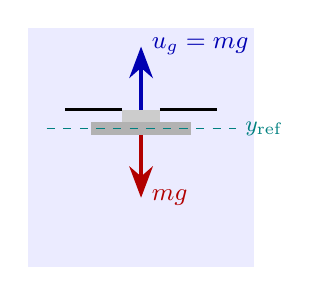
\begin{tikzpicture}[scale=0.8]
  \fill[blue!8] (-1.8,-0.3) rectangle (1.8,3.5);
  % Drone body
  \fill[gray!60] (-0.8,1.8) rectangle (0.8,2.0);
  \fill[gray!40] (-0.3,2.0) rectangle (0.3,2.2);
  % Propellers
  \draw[thick] (-1.2,2.2) -- (-0.3,2.2);
  \draw[thick] (0.3,2.2) -- (1.2,2.2);
  % Forces
  \draw[-{Stealth[length=4mm]},red!70!black,very thick] (0,1.8) -- (0,0.8) node[right,font=\small] {$mg$};
  \draw[-{Stealth[length=4mm]},blue!70!black,very thick] (0,2.2) -- (0,3.2) node[right,font=\small] {$u_g = mg$};
  % Reference line
  \draw[dashed,teal] (-1.5,1.9) -- (1.5,1.9) node[right,font=\footnotesize] {$y_{\mathrm{ref}}$};
\end{tikzpicture}
\end{column}
\end{columns}
\end{frame}

% ==============================================================
\begin{frame}[shrink=5]{Case Study: Magnetic Levitation}

\begin{columns}[T]
\begin{column}{0.45\textwidth}
\begin{block}{System}
\begin{itemize}
  \item Electromagnet suspends steel ball
  \item State: gap $y$ and velocity $\dot{y}$
  \item Input: coil current $u$
  \item \textbf{Open-loop unstable}
  \item Nonlinear: $\ddot{y} = g - \frac{C}{m}\!\left(\frac{u}{y}\right)^{\!2}$
\end{itemize}
\end{block}

\begin{block}{LQR design}
\begin{enumerate}
  \item Linearise around equilibrium gap $y_{\text{eq}}$
  \item Compute $u_g = y_{\text{eq}}\sqrt{mg/C}$
  \item Design LQR on linearised model
  \item Apply affine law to \textbf{nonlinear} plant
\end{enumerate}
\end{block}
\end{column}

\begin{column}{0.52\textwidth}
% MagLev schematic
\centering
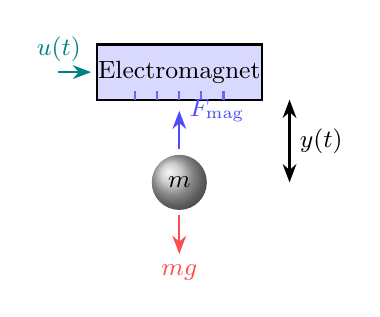
\begin{tikzpicture}[scale=0.7]
  % Electromagnet
  \fill[blue!15] (-1.5,3) rectangle (1.5,4);
  \draw[thick] (-1.5,3) rectangle (1.5,4);
  \node[font=\small] at (0,3.5) {Electromagnet};
  % Coil symbol
  \foreach \i in {-0.8,-0.4,0,0.4,0.8} {
    \draw[thick,blue!60] (\i,3) -- (\i,3.15);
  }
  % Gap annotation
  \draw[{Stealth}-{Stealth},thick] (2,1.5) -- node[right,font=\small] {$y(t)$} (2,3);
  % Ball
  \shade[ball color=gray!50] (0,1.5) circle (0.5);
  \node[font=\small] at (0,1.5) {$m$};
  % Forces
  \draw[-{Stealth},red!70,thick] (0,0.9) -- (0,0.2) node[below,font=\small] {$mg$};
  \draw[-{Stealth},blue!70,thick] (0,2.1) -- (0,2.8) node[right,font=\small] {$F_{\text{mag}}$};
  % Current
  \draw[-{Stealth},teal,thick] (-2.2,3.5) -- (-1.6,3.5) node[above left,font=\small] {$u(t)$};
\end{tikzpicture}
\end{column}
\end{columns}
\end{frame}

% ==============================================================
\begin{frame}{MagLev Results: Setpoint Tracking}
\centering
\includegraphicssafe[width=0.65\textwidth]{Figures/Maglev}

\smallskip
{\small Gap transitions smoothly from 10\,mm to 12\,mm with no overshoot.\\
Control current settles to a \textbf{non-zero} steady-state value --- the feedforward component $u_g$.\\[3pt]
\textbf{Limitation:} LQR does not enforce current limits or gap safety bounds $\Rightarrow$ need MPC.}
\end{frame}

% ==============================================================
\begin{frame}[shrink=5]{LQR Summary}
\begin{center}
\renewcommand{\arraystretch}{1.3}
\begin{tabular}{l l}
\toprule
\textbf{Concept} & \textbf{Key result} \\
\midrule
Finite-horizon LQR & Time-varying gains $K_k$ via Riccati backward pass \\
Infinite-horizon LQR & Constant gain $K$ from DARE: \texttt{[P,L,K] = dare(A,B,Q,R)} \\
Stability & Closed-loop $A - BK$ has all eigenvalues inside unit circle \\
Setpoint tracking & Affine law: $u_k = u_g - K(x_k - x_g)$ \\
Weight tuning & $Q_{ii} = 1/(\max x_i)^2$, \; $R_{jj} = 1/(\max u_j)^2$ \\
Bridge to MPC & Same QP, just add inequality constraints $Gz \le h$ \\
\bottomrule
\end{tabular}
\end{center}

\begin{alertblock}{What LQR cannot do}
\begin{itemize}
  \item Handle actuator saturation or safety constraints
  \item Handle unknown disturbances (no integral action)
  \item Work with unmeasured states (needs full state $x_k$)
\end{itemize}
$\Rightarrow$ Kalman Filter addresses the last point. MPC addresses all three.
\end{alertblock}
\end{frame}


% %%%%%%%%%%%%%%%%%%%%%%%%%%%%%%%%%%%%%%%%%%%%%%%%%%%%%%%%%%%%%%
% PART II: KALMAN FILTER
% %%%%%%%%%%%%%%%%%%%%%%%%%%%%%%%%%%%%%%%%%%%%%%%%%%%%%%%%%%%%%%
\begin{frame}{}
\centering
\vfill
{\Huge\bfseries Part II}\\[12pt]
{\Large The Kalman Filter}\\[6pt]
{\normalsize Chapter 6}
\vfill
\end{frame}

% ==============================================================
\begin{frame}[shrink=3]{Kalman Filter Problem Statement}
\begin{block}{Stochastic system}
\[
  x_{k+1} = A\,x_k + B\,u_k + w_k, \qquad w_k \sim \mathcal{N}(0, W)
\]
\[
  y_k = C\,x_k + v_k, \qquad\qquad\qquad\;\; v_k \sim \mathcal{N}(0, V)
\]
\begin{itemize}
  \item $w_k$: process noise (model uncertainty, disturbances)
  \item $v_k$: measurement noise (sensor imperfection)
  \item $w_k$ and $v_k$ are white, zero-mean, mutually independent
\end{itemize}
\end{block}

\begin{block}{Objective}
At each step $k$, compute the \textbf{best estimate} $\hat{x}_k$ of the true state $x_k$,
using only the available measurements $y_1, y_2, \ldots, y_k$ and known inputs $u_0, \ldots, u_{k-1}$.

\medskip
``Best'' $=$ minimise the mean-squared estimation error:
$\quad \min\; \mathbb{E}\bigl[\|x_k - \hat{x}_k\|^2\bigr]$.
\end{block}
\end{frame}

% ==============================================================
\begin{frame}{Key idea: Predict, then Correct}

\centering
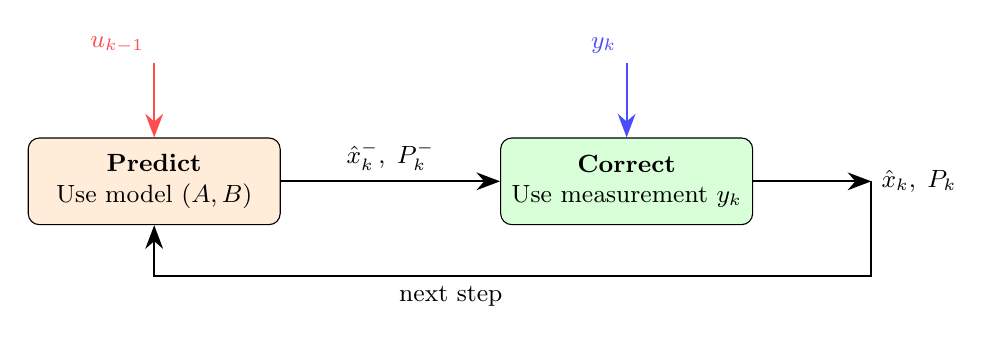
\begin{tikzpicture}[
  box/.style={draw,rounded corners,minimum width=3.2cm,minimum height=1.1cm,
              align=center,font=\small},
  arr/.style={-{Stealth[length=3mm]},thick}
]
  % Predict
  \node[box,fill=orange!15] (pred) at (0,0) {\textbf{Predict}\\Use model $(A,B)$};
  % Correct
  \node[box,fill=green!15]  (corr) at (6,0) {\textbf{Correct}\\Use measurement $y_k$};
  % Arrows
  \draw[arr] (pred) -- node[above,font=\small] {$\hat{x}_k^-,\; P_k^-$} (corr);
  \draw[arr] (corr.east) -- ++(1.5,0) node[right,font=\small] {$\hat{x}_k,\; P_k$};
  \draw[arr] (corr.east)++(1.5,0) -- ++(0,-1.2) -| (pred.south) node[below left,font=\small,pos=0.25] {next step};
  % Measurement
  \draw[arr,blue!70] (6,1.5) -- (corr.north) node[above left,font=\small,pos=0] {$y_k$};
  % Input
  \draw[arr,red!70] (0,1.5) -- (pred.north) node[above left,font=\small,pos=0] {$u_{k-1}$};
\end{tikzpicture}

\vspace{12pt}

\begin{columns}[T]
\begin{column}{0.45\textwidth}
\begin{block}{Predict (time update)}
Propagate state and uncertainty forward using the \textbf{model}
\end{block}
\end{column}
\begin{column}{0.45\textwidth}
\begin{block}{Correct (measurement update)}
Blend prediction with new \textbf{measurement} via the Kalman gain $L_k$
\end{block}
\end{column}
\end{columns}
\end{frame}

% ==============================================================
\begin{frame}[shrink=5]{Algorithm: The Discrete Kalman Filter}
\begin{block}{Algorithm --- Discrete-Time Kalman Filter}
\textbf{Input:} $A, B, C, W, V, \hat{x}_0, P_0$. \quad \textbf{Output:} State estimates $\hat{x}_k$ at each step.

\medskip
At each time step $k$:

\medskip
\textbf{1. Predict:}
\[
  \hat{x}_k^- = A\,\hat{x}_{k-1} + B\,u_{k-1}, \qquad
  P_k^- = A\,P_{k-1}\,A^\T + W
\]

\textbf{2. Compute Kalman Gain:}
\[
  S_k = C\,P_k^-\,C^\T + V, \qquad
  L_k = P_k^-\,C^\T\,S_k^{-1}
\]

\textbf{3. Correct:}
\[
  \hat{x}_k = \hat{x}_k^- + L_k\underbrace{\bigl(y_k - C\,\hat{x}_k^-\bigr)}_{\text{innovation } \tilde{y}_k}, \qquad
  P_k = (I - L_k\,C)\,P_k^-
\]
\end{block}

\smallskip
{\small $S_k$: innovation covariance. \; $L_k$: optimal blending weight between model and measurement.}
\end{frame}

% ==============================================================
\begin{frame}[shrink=3]{Innovation: the information content of a measurement}

\begin{block}{Definition}
\[
  \tilde{y}_k = y_k - C\,\hat{x}_k^- \qquad \text{(measurement $-$ predicted measurement)}
\]
\end{block}

\begin{itemize}
  \item If $\tilde{y}_k \approx 0$: measurement confirms our prediction $\Rightarrow$ small correction
  \item If $\tilde{y}_k$ is large: measurement disagrees $\Rightarrow$ large correction
  \item The gain $L_k$ scales \emph{how much} we trust this disagreement
\end{itemize}

\begin{exampleblock}{Analogy}
\begin{itemize}
  \item \textbf{High $W$ / Low $V$} (noisy model, good sensor): $L_k$ is large $\Rightarrow$ trust measurement
  \item \textbf{Low $W$ / High $V$} (good model, noisy sensor): $L_k$ is small $\Rightarrow$ trust model
\end{itemize}
The Kalman filter automatically computes this trade-off optimally at each step.
\end{exampleblock}
\end{frame}

% ==============================================================
\begin{frame}[shrink=5]{Steady-State Kalman Filter}
\begin{block}{Key result}
For LTI systems, if $(A, C)$ is \textbf{detectable} and $(A, W^{1/2})$ is \textbf{stabilisable},
the covariance $P_k$ converges to a constant $P_\infty$ satisfying:
\[
  P_\infty = A\,P_\infty\,A^\T + W - A\,P_\infty\,C^\T\!\bigl(C\,P_\infty\,C^\T + V\bigr)^{-1}\!C\,P_\infty\,A^\T
\]
This is the \textbf{estimation DARE} --- same equation structure as the LQR DARE!
\end{block}

\begin{block}{Constant gain filter}
\[
  L = P_\infty\,C^\T\!\bigl(C\,P_\infty\,C^\T + V\bigr)^{-1}
\]
\begin{itemize}
  \item No need to propagate $P_k$ online --- just use constant $L$
  \item Identical to a \textbf{Luenberger observer} with optimal gain
  \item Compute once offline via \texttt{dare(A', C', W, V)}
\end{itemize}
\end{block}
\end{frame}

% ==============================================================
\begin{frame}{Duality: LQR $\longleftrightarrow$ Kalman Filter}
\begin{center}
\renewcommand{\arraystretch}{1.4}
\begin{tabular}{l c c}
\toprule
& \textbf{LQR (Control)} & \textbf{Kalman Filter (Estimation)} \\
\midrule
Direction   & Backward (Riccati)     & Forward (recursive) \\
Dynamics    & $A$                    & $A^\T$ \\
Actuation / Sensing & $B$           & $C^\T$ \\
State penalty / Process noise & $Q$ & $W$ \\
Input penalty / Meas.\ noise & $R$  & $V$ \\
Result      & Feedback gain $K$      & Observer gain $L$ \\
DARE call   & \texttt{dare(A,B,Q,R)} & \texttt{dare(A',C',W,V)} \\
\bottomrule
\end{tabular}
\end{center}

\begin{alertblock}{Practical consequence}
If you can solve one, you can solve the other --- same algorithm, different inputs.
MATLAB's \texttt{dare()} handles both.
\end{alertblock}
\end{frame}

% ==============================================================
\begin{frame}[fragile,shrink=3]{MATLAB: Steady-State Kalman Filter}
\begin{lstlisting}[style=matlab]
% System: double integrator, observe position only
dt = 0.1;
A = [1, dt; 0, 1];   B = [0.5*dt^2; dt];
C = [1, 0];                        % measure position only

W = 1e-4 * eye(2);                 % process noise covariance
V = 1e-2;                          % measurement noise variance

% Steady-state Kalman gain via duality
[P_ss, ~, ~] = dare(A', C', W, V);
L = P_ss * C' / (C * P_ss * C' + V);

fprintf('Kalman gain L = [%.4f; %.4f]\n', L);
\end{lstlisting}

\begin{block}{One-step form (Luenberger-style)}
\[
  \hat{x}_{k+1} = A\,\hat{x}_k + B\,u_k + \underbrace{A\,L}_{\text{observer gain}}\bigl(y_k - C\,\hat{x}_k\bigr)
\]
\end{block}
\end{frame}

% ==============================================================
\begin{frame}{Example: Estimating Position and Velocity}
\centering
\includegraphicssafe[width=0.58\textwidth]{Figures/Kalman_Performance}

\smallskip
{\scriptsize (a) Filter smooths noisy position data.\;
(b) Velocity reconstructed from position only.\;
(c) Error within $\pm 3\sigma$ bounds.}
\end{frame}

% ==============================================================
\begin{frame}[shrink=5]{Practical Tuning: Selecting $W$ and $V$}
\begin{block}{Measurement noise $V$}
\begin{itemize}
  \item Usually \textbf{known} from sensor datasheets or calibration experiments
  \item Record sensor data while stationary $\Rightarrow$ compute sample variance
  \item Diagonal $V$ if sensors are independent
\end{itemize}
\end{block}

\begin{block}{Process noise $W$ --- the main tuning knob}
\begin{itemize}
  \item Lumps \textbf{all model uncertainty}: unmodelled dynamics, disturbances, parameter errors
  \item Rarely known precisely --- treat as a \textbf{design parameter}
\end{itemize}
\end{block}

\begin{center}
\renewcommand{\arraystretch}{1.2}
\begin{tabular}{l l l}
\toprule
$W$ & Filter behaviour & When to use \\
\midrule
\textbf{Large} $W$ & Responsive, noisy estimates & Fast-changing dynamics, poor model \\
\textbf{Small} $W$ & Smooth, slow estimates & Slowly changing dynamics, good model \\
\bottomrule
\end{tabular}
\end{center}

\smallskip
{\small \textbf{Rule of thumb:} Start with $W = \alpha I$, vary $\alpha$ over decades ($10^{-6}$ to $10^{0}$), examine estimation error on validation data.}
\end{frame}


% %%%%%%%%%%%%%%%%%%%%%%%%%%%%%%%%%%%%%%%%%%%%%%%%%%%%%%%%%%%%%%
% PART III: LQG
% %%%%%%%%%%%%%%%%%%%%%%%%%%%%%%%%%%%%%%%%%%%%%%%%%%%%%%%%%%%%%%
\begin{frame}{}
\centering
\vfill
{\Huge\bfseries Part III}\\[12pt]
{\Large LQG: Combining LQR + Kalman Filter}\\[6pt]
{\normalsize The Separation Principle}
\vfill
\end{frame}

% ==============================================================
\begin{frame}[shrink=5]{LQG = LQR + Kalman Filter}
\begin{block}{The Separation Principle}
For linear systems with Gaussian noise, the optimal output-feedback controller decomposes into two independent problems:
\begin{enumerate}
  \item \textbf{Estimation:} Design Kalman filter as if control were known
  \item \textbf{Control:} Design LQR as if true state were known
\end{enumerate}
The combined controller $u_k = -K\,\hat{x}_k$ is \textbf{optimal} among all linear output-feedback laws.
\end{block}

\centering
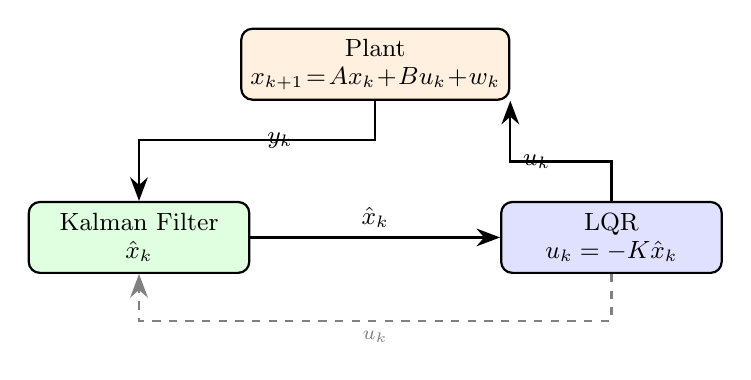
\begin{tikzpicture}[
  box/.style={draw,thick,rounded corners,minimum width=2.8cm,minimum height=0.9cm,
              align=center,font=\small},
  arr/.style={-{Stealth[length=3mm]},thick}
]
  % Nodes: Plant top-centre, KF bottom-left, LQR bottom-right
  \node[box,fill=orange!12] (plant) at (3,0)     {Plant\\[-1pt]$x_{k+1}\!=\!Ax_k\!+\!Bu_k\!+\!w_k$};
  \node[box,fill=green!12]  (kf)    at (0,-2.2)  {Kalman Filter\\[-1pt]$\hat{x}_k$};
  \node[box,fill=blue!12]   (lqr)   at (6,-2.2)  {LQR\\[-1pt]$u_k = -K\hat{x}_k$};

  % y_k: Plant → down-left → Kalman Filter
  \draw[arr] (plant.south) -- ++(0,-0.5) -| node[pos=0.25,right,font=\small] {$y_k$} (kf.north);

  % x_hat: Kalman Filter → LQR
  \draw[arr] (kf.east) -- node[above,font=\small] {$\hat{x}_k$} (lqr.west);

  % u_k: LQR → up-right → Plant
  \draw[arr] (lqr.north) -- ++(0,0.5) -| node[pos=0.25,left,font=\small] {$u_k$} (plant.south east);

  % u_k (dashed): LQR → Kalman Filter (the filter also needs u_k)
  \draw[arr,dashed,gray] (lqr.south) -- ++(0,-0.6) -| node[below,pos=0.25,font=\scriptsize,gray] {$u_k$} (kf.south);
\end{tikzpicture}
\end{frame}

% ==============================================================
\begin{frame}[fragile,shrink=10]{MATLAB: Complete LQG Controller}
\begin{lstlisting}[style=matlab]
% System
dt = 0.1;
A = [1, dt; 0, 1];  B = [0.5*dt^2; dt];  C = [1, 0];
Q = eye(2);  R = 0.1;  W = 1e-4*eye(2);  V = 1e-2;

% LQR gain
[~, ~, K] = dare(A, B, Q, R);

% Kalman gain
[P_ss, ~, ~] = dare(A', C', W, V);
L = P_ss * C' / (C * P_ss * C' + V);

% Simulate LQG
x = [1; 0];  xhat = [0; 0];       % true state, estimate
for k = 1:200
    y = C*x + sqrt(V)*randn;      % noisy measurement

    % Kalman update
    xhat_pred = A*xhat + B*u;
    xhat = xhat_pred + L*(y - C*xhat_pred);

    % LQR control using estimate
    u = -K * xhat;

    % Plant update
    x = A*x + B*u + sqrtm(W)*randn(2,1);
end
\end{lstlisting}
\end{frame}


% %%%%%%%%%%%%%%%%%%%%%%%%%%%%%%%%%%%%%%%%%%%%%%%%%%%%%%%%%%%%%%
% PART IV: PRACTICAL CALIBRATION
% %%%%%%%%%%%%%%%%%%%%%%%%%%%%%%%%%%%%%%%%%%%%%%%%%%%%%%%%%%%%%%
\begin{frame}{}
\centering
\vfill
{\Huge\bfseries Part IV}\\[12pt]
{\Large Practical Calibration Remarks}
\vfill
\end{frame}

% ==============================================================
\begin{frame}[shrink=5]{LQR Calibration Checklist}

\begin{enumerate}
  \item \textbf{Normalise weights.}
    Set $Q_{ii} = 1/(\max x_i)^2$, $R_{jj} = 1/(\max u_j)^2$.

  \item \textbf{Adjust $Q/R$ ratio.}
    \begin{itemize}
      \item Increase $Q/R$ for faster response (more aggressive input)
      \item Decrease $Q/R$ for smoother, energy-efficient response
    \end{itemize}

  \item \textbf{Check eigenvalues.}
    Verify $|\lambda_i(A - BK)| < 1$.  Eigenvalues near 0 $=$ fast but sensitive.  Near 1 $=$ slow but robust.

  \item \textbf{Simulate before deploying.}
    Apply to nonlinear model (RK4 simulation) to verify local validity.

  \item \textbf{Add setpoint feedforward.}
    Always compute $(x_g, u_g)$ --- never rely on feedback alone for tracking.
\end{enumerate}

\begin{alertblock}{Common pitfall}
Forgetting that LQR assumes \textbf{no constraints}. If the resulting $u_k$ exceeds actuator limits, the closed-loop performance degrades or becomes unstable. $\Rightarrow$ use MPC.
\end{alertblock}
\end{frame}

% ==============================================================
\begin{frame}[shrink=5]{Kalman Filter Calibration Checklist}

\begin{enumerate}
  \item \textbf{Measure $V$ from data.}
    Record sensor output with system stationary; compute sample covariance.

  \item \textbf{Start with $W = \alpha I$.}
    Use $\alpha = 10^{-4}$ as initial guess.  Increase $\alpha$ if estimates lag; decrease if too noisy.

  \item \textbf{Check innovation statistics.}
    If the filter is well-tuned, innovations $\tilde{y}_k$ should be:
    \begin{itemize}
      \item Zero-mean
      \item White (uncorrelated over time)
      \item Consistent with predicted covariance $S_k$
    \end{itemize}

  \item \textbf{Verify observability.}
    Rank of $\mathcal{O} = [C;\; CA;\; CA^2;\; \ldots;\; CA^{n-1}]$ must equal $n$.

  \item \textbf{Validate on separate data.}
    Never tune on the same data you test on.
\end{enumerate}

\begin{exampleblock}{Sensor fusion intuition}
If you have a fast but noisy sensor (e.g.\ accelerometer) and a slow but accurate sensor (e.g.\ GPS), the Kalman filter automatically blends them: accelerometer for high-frequency, GPS for low-frequency drift correction.
\end{exampleblock}
\end{frame}


% ==============================================================
\begin{frame}[shrink=5]{Summary: From LQR to MPC}

\begin{center}
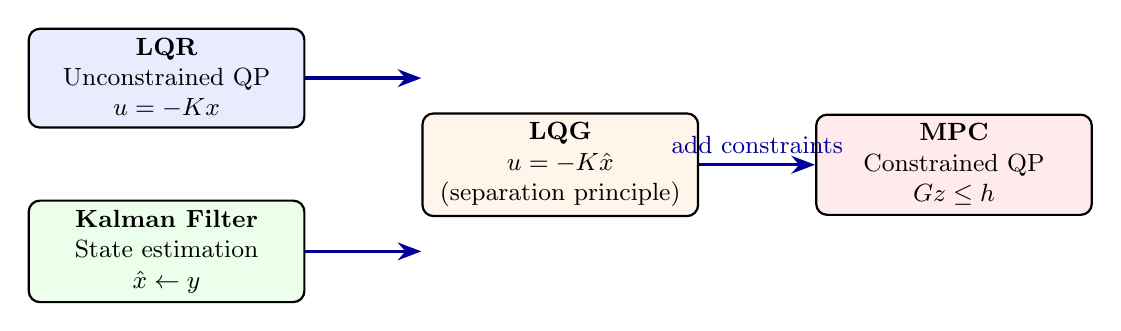
\begin{tikzpicture}[
  box/.style={draw,thick,rounded corners=4pt,minimum width=3.5cm,minimum height=1cm,
              align=center,font=\small},
  arr/.style={-{Stealth[length=3mm]},very thick,blue!60!black}
]
  \node[box,fill=blue!8]   (lqr) at (0,0)    {\textbf{LQR}\\Unconstrained QP\\$u = -Kx$};
  \node[box,fill=green!8]  (kf)  at (0,-2.2) {\textbf{Kalman Filter}\\State estimation\\$\hat{x} \leftarrow y$};
  \node[box,fill=orange!8] (lqg) at (5,-1.1) {\textbf{LQG}\\$u = -K\hat{x}$\\(separation principle)};
  \node[box,fill=red!8]    (mpc) at (10,-1.1) {\textbf{MPC}\\Constrained QP\\$Gz \le h$};

  \draw[arr] (lqr.east) -- (lqg.west |- lqr.east);
  \draw[arr] (kf.east)  -- (lqg.west |- kf.east);
  \draw[arr] (lqg) -- node[above,font=\small] {add constraints} (mpc);
\end{tikzpicture}
\end{center}

\vspace{6pt}

\begin{block}{Key takeaways}
\begin{itemize}
  \item LQR and Kalman filter are \textbf{dual problems} solved by the same DARE
  \item LQG combines them optimally via the separation principle
  \item MPC = LQR's QP formulation + inequality constraints + receding horizon
  \item Weight tuning ($Q, R, W, V$) follows the same principles in LQR, Kalman, and MPC
\end{itemize}
\end{block}
\end{frame}

% ==============================================================
\begin{frame}[shrink=10]{Self-study}
\begin{block}{Read in the textbook}
\begin{itemize}
  \item Chapter 5: Derivation of Riccati recursion from KKT conditions (Sections 5.2--5.3)
  \item Chapter 5: DARE convergence proof and stability guarantee (Section 5.5)
  \item Chapter 6: Optimal Kalman gain derivation from MSE minimisation (Section 6.3)
  \item Chapter 6: Joseph form for numerical stability (Section 6.3)
\end{itemize}
\end{block}

\begin{block}{Exercises}
\begin{enumerate}
  \item Simulate the double integrator with three different $(Q, R)$ pairs.  Compare settling time and peak input.
  \item For the MagLev system, what happens if you do \textbf{not} include the feedforward term $u_g$?
  \item Implement the full LQG controller for a double integrator with position-only measurement.  Vary $W$ over $[10^{-6}, 10^{0}]$ and plot the estimation error.
  \item Verify the duality: solve the Kalman DARE using \texttt{dare(A',C',W,V)} and confirm $L$ matches the manual formula.
\end{enumerate}
\end{block}
\end{frame}

\end{document}
